\chapter{De hersenen aan het commando}\label{ch:g5:brain-in-command}

Er vliegt een bal op je af; je vangt hem. Een halve seconde, geen enkele
gedachte --- en toch hebben je \omterm{def:g1:the-five-senses:sense}{ogen} in die halve seconde een vliegend
voorwerp gemeld, heeft iets zijn baan berekend, en zijn tientallen
\omterm{def:g3:bones-and-muscles:muscle}{spieren} tot precies de juiste vangbeweging bevolen. Dat iets zijn de
\omterm{def:g5:brain-in-command:system}{hersenen}, en dit hoofdstuk volgt hun bevelen door de bedrading van het
lichaam.

\section{Het commandonetwerk}

\begin{definition}[Het zenuwstelsel]\label{def:g5:brain-in-command:system}
Het \emph{zenuwstelsel}\index{zenuwstelsel} is het commandonetwerk van
het lichaam:
\begin{itemize}
  \item de \emph{hersenen}\index{hersenen}, beschut door de \omterm{def:g3:bones-and-muscles:skeleton}{schedel}
        (\cref{def:g3:bones-and-muscles:skeleton}), vormen het centrum:
        ze ontvangen alle meldingen en geven alle bevelen;
  \item het \emph{ruggenmerg}\index{ruggenmerg}, een dikke kabel van
        zenuwweefsel, loopt van de hersenen omlaag binnen de
        beschermende zuil van de \omterm{def:g3:bones-and-muscles:skeleton}{wervelkolom};
  \item de \emph{zenuwen}\index{zenuw}, witte draden die vanuit hersenen
        en ruggenmerg naar elk orgaan vertakken, dragen de boodschappen
        --- bij de snelste met meer dan \qty{100}{m/s}.
\end{itemize}
\end{definition}

\begin{proposition}[Melden, beslissen, bevelen]\label{prop:g5:brain-in-command:loop}
Elke handeling doorloopt dezelfde lus
(\cref{prop:g1:the-five-senses:brain} was er de eerste schets van):
\begin{enumerate}
  \item de \emph{zintuigorganen} melden: \omterm{def:g5:brain-in-command:system}{zenuwen} dragen hun
        boodschappen \emph{naar} de \omterm{def:g5:brain-in-command:system}{hersenen};
  \item de \emph{\omterm{def:g5:brain-in-command:system}{hersenen}} voegen de meldingen samen, beslissen en
        stellen bevelen op;
  \item \omterm{def:g5:brain-in-command:system}{zenuwen} dragen de bevelen \emph{van} de \omterm{def:g5:brain-in-command:system}{hersenen} naar de
        \emph{\omterm{def:g3:bones-and-muscles:muscle}{spieren}} (\cref{def:g3:bones-and-muscles:muscle}), die op
        bevel \omterm{def:g3:bones-and-muscles:muscle}{samentrekken}.
\end{enumerate}
Zintuigorganen melden, \omterm{def:g3:bones-and-muscles:muscle}{spieren} gehoorzamen --- geen van beide beslist ooit.
\end{proposition}
\admitted

\begin{omfigure}
\begin{tikzpicture}
  % eye
  \draw[thick] (-0.7,1.7) ellipse (0.5 and 0.28);
  \fill[omDef] (-0.58,1.7) circle (0.13);
  \node[font=\small, align=center] (eye) at (-0.7,0.85)
    {het oog ziet\\ de bal};
  % brain
  \draw[thick, omDef, fill=omDef!8, rounded corners=8pt]
    (3.2,1.15) rectangle (6.4,2.45);
  \node[font=\small\bfseries, omDef] at (4.8,2.05) {de hersenen};
  \node[font=\footnotesize] at (4.8,1.55) {beslissen tot de vangbeweging};
  % muscle
  \draw[thick, omThm, fill=omThm!15]
    (9.6,1.5) .. controls (10.0,1.85) and (10.6,1.85) .. (11.0,1.55)
    .. controls (10.6,1.35) and (10.0,1.35) .. (9.6,1.5);
  \node[font=\small, align=center] at (10.3,0.85)
    {de armspieren\\ trekken samen};
  % arrows
  \draw[->, very thick, omMeth] (-0.1,1.7) -- (3.1,1.8)
    node[pos=0.42, above=2pt, font=\footnotesize, omMeth]
    {melding, langs een zenuw};
  \draw[->, very thick, omProp] (6.5,1.8) -- (9.5,1.6)
    node[pos=0.5, above=2pt, font=\footnotesize, omProp]
    {bevel, langs een zenuw};
\end{tikzpicture}

{\small De lus van elke handeling: melding naar de \omterm{def:g5:brain-in-command:system}{hersenen}, beslissing,
bevel naar de \omterm{def:g3:bones-and-muscles:muscle}{spieren}.}
\end{omfigure}

\begin{example}[De vangbeweging, langzaam afgespeeld]\label{ex:g5:brain-in-command:catch}
Speel die halve seconde langzaam af: de \omterm{def:g1:the-five-senses:sense}{ogen} volgen de bal en melden,
onafgebroken; de \omterm{def:g5:brain-in-command:system}{hersenen} leiden uit melding na melding af waar de bal
zal zijn; bevelen stromen naar de \omterm{def:g1:my-body:parts}{benen} (een stap naar links), de \omterm{def:g1:my-body:parts}{romp}
(leunen), de \omterm{def:g1:my-body:parts}{arm} en de vingers (open --- nu dicht). Geen enkel orgaan
``ving de bal'': \omterm{def:g1:the-five-senses:sense}{ogen}, \omterm{def:g5:brain-in-command:system}{hersenen} en \omterm{def:g3:bones-and-muscles:muscle}{spieren} speelden elk hun regel uit
\cref{prop:g5:brain-in-command:loop}.
\end{example}

\begin{remark}[Meer dan bewegen]\label{rem:g5:brain-in-command:more}
Dezelfde \omterm{def:g5:brain-in-command:system}{hersenen} die ballen vangen bewaren ook je herinneringen, houden
je aandacht op deze bladzijde, dromen 's nachts --- en draaien diensten
waar je nooit bij stilstaat: ze houden de ademhaling dag en nacht op
gang (\cref{def:g4:breathing:movements}) en stemmen het tempo van het
\omterm{def:g4:heart-and-blood:heart}{hart} af op wat het lichaam nodig heeft
(\cref{ex:g4:heart-and-blood:effort}). Sommige bevelen geef jij; andere
geven de \omterm{def:g5:brain-in-command:system}{hersenen} voor jou.
\end{remark}

\section{De lus meten: de reactietijd}

\begin{definition}[Reactietijd]\label{def:g5:brain-in-command:reaction}
De lus is snel maar niet ogenblikkelijk: melding, beslissing en bevel
nemen elk hun deel. De vertraging tussen een signaal en de reactie van
het lichaam is de \emph{reactietijd}\index{reactietijd} --- bij een
eenvoudige taak (vangen, drukken, grijpen) ongeveer een vijfde seconde
bij een geoefend persoon, iets meer bij kinderen.
\end{definition}

\begin{method}[De liniaalproef]\label{met:g5:brain-in-command:ruler}
\omterm{def:g5:brain-in-command:reaction}{Reactietijd} zonder ander instrument dan een liniaal:
\begin{enumerate}
  \item een partner houdt een liniaal verticaal hangend, met de
        nulstreep omlaag, tussen je open duim en vinger;
  \item zonder waarschuwing laat de partner los; jij vangt de liniaal zo
        snel als je kunt;
  \item lees af waar je hem gevangen hebt: hoe minder centimeters er
        voorbijgegleden zijn, hoe sneller jouw lus;
  \item herhaal het een paar keer en houd je gebruikelijke waarde aan
        --- losse pogingen springen alle kanten op.
\end{enumerate}
De vallende liniaal zet tijd om in centimeters: ongeveer
$\qty{15}{cm}$ komt overeen met een zesde seconde.
\end{method}

\begin{omfigure}
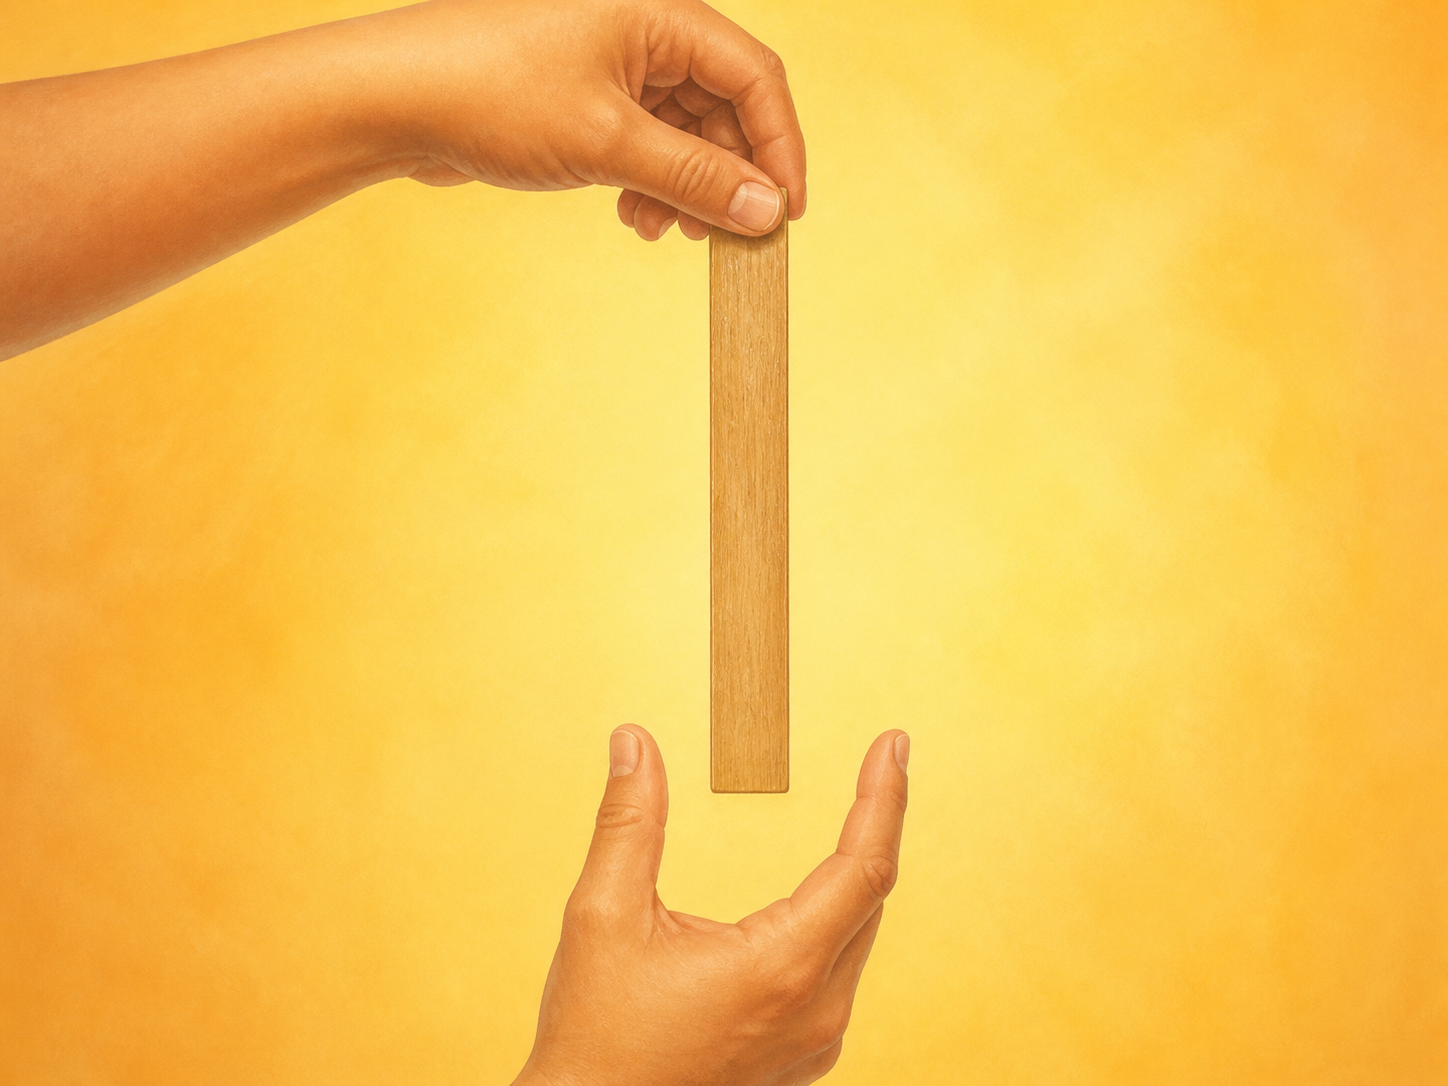
\includegraphics[width=0.5\linewidth]{images/book1/ai/g5-brain-ruler.png}

{\small De liniaalproef, een ogenblik voor de val: als de bovenste hand
loslaat, begint de lus van de onderste --- zien, beslissen, sluiten ---
aan haar vijfde seconde.}
\end{omfigure}

\begin{example}[Waarom de bijrijder het eerst naar adem hapt]\label{ex:g5:brain-in-command:driver}
Een vijfde seconde lijkt niets --- tot snelheid het vermenigvuldigt. Een
auto legt op snelwegsnelheid ongeveer \qty{7}{m} af tijdens een reactie
van een vijfde seconde: de bestuurder heeft de rem nog niet aangeraakt,
en de auto is een klaslokaal doorgestoken. De \omterm{def:g5:brain-in-command:reaction}{reactietijd} is de reden
dat er afstanden tussen auto's bestaan, en dat de aandacht van een
bestuurder een veiligheidsorgaan is.
\end{example}

\begin{remark}[De lus trainen]\label{rem:g5:brain-in-command:training}
Oefening verkort en verscherpt de lus --- niet de snelheid van de
\omterm{def:g5:brain-in-command:system}{zenuwen}, maar de wegwijzers van de \omterm{def:g5:brain-in-command:system}{hersenen}. De beginnende jongleur laat
alles vallen; een maand later sturen dezelfde \omterm{def:g5:brain-in-command:system}{hersenen} dezelfde handen
zonder zichtbare moeite door drie ballen heen. Een vaardigheid leren is
de \omterm{def:g5:brain-in-command:system}{hersenen} betere paden laten aanleggen --- nog iets dat met oefening
groeit, net als de \omterm{def:g3:bones-and-muscles:muscle}{spieren} uit
\cref{met:g3:bones-and-muscles:care}.
\end{remark}

\section{De commandant beschermen}

\begin{proposition}[Slaap, voedsel, veiligheid]\label{prop:g5:brain-in-command:protect}
De \omterm{def:g5:brain-in-command:system}{hersenen} zijn het best beschermde orgaan van het lichaam --- helm van
de \omterm{def:g3:bones-and-muscles:skeleton}{schedel}, zuil van de \omterm{def:g3:bones-and-muscles:skeleton}{wervelkolom} --- en het meest veeleisende: hoewel
ze maar een klein deel van het lichaamsgewicht vormen, verbruiken ze een
groot deel van de \omterm{prop:g3:balanced-diet:jobs}{energie} en de zuurstof
(\cref{prop:g4:heart-and-blood:carries}), en ze doen hun opruimwerk en
herstel tijdens de \emph{\omterm{prop:g1:healthy-habits:needs}{slaap}}
(\cref{prop:g1:healthy-habits:needs}). Vermoeide \omterm{def:g5:brain-in-command:system}{hersenen} commanderen
slecht: tragere reacties, verstrooide aandacht, chagrijnige beslissingen.
\end{proposition}
\admitted

\begin{example}[Helmen zijn er voor de lus]\label{ex:g5:brain-in-command:helmet}
\omterm{def:g3:bones-and-muscles:skeleton}{Botten} genezen (\cref{rem:g3:bones-and-muscles:alive}); het weefsel van
de \omterm{def:g5:brain-in-command:system}{hersenen} doet dat, eenmaal ernstig beschadigd, meestal niet. Dat is
de rekensom achter fietshelmen: \omterm{def:g3:bones-and-muscles:skeleton}{schedel} plus schuim waar de eigen
bescherming van het lichaam misschien niet genoeg is. Goedkope
verzekering voor het orgaan dat al het andere aanstuurt.
\end{example}

\section{Oefeningen}

\begin{exercise}[$\star$]\label{exo:g5:brain-in-command:1}
Noem de drie delen van het \omterm{def:g5:brain-in-command:system}{zenuwstelsel} en de rol van elk.
\end{exercise}

\begin{exercise}[$\star$]\label{exo:g5:brain-in-command:2}
Beschrijf de lus van elke handeling in drie stappen. Welke delen melden,
welk deel beslist, welke gehoorzamen?
\end{exercise}

\begin{exercise}[$\star$]\label{exo:g5:brain-in-command:3}
Waar worden de \omterm{def:g5:brain-in-command:system}{hersenen} en het \omterm{def:g5:brain-in-command:system}{ruggenmerg} elk beschermd, en door welke
\omterm{def:g3:bones-and-muscles:skeleton}{botten}?
\end{exercise}

\begin{exercise}[$\star$]\label{exo:g5:brain-in-command:4}
Wat is de \omterm{def:g5:brain-in-command:reaction}{reactietijd}? Geef haar ruwe waarde voor een eenvoudige taak.
\end{exercise}

\begin{exercise}[$\star$]\label{exo:g5:brain-in-command:5}
Speel langzaam af, zoals in \cref{ex:g5:brain-in-command:catch}: je stapt
op iets scherps en je voet trekt zich terug. Wie meldde, wie besliste,
wie gehoorzaamde?
\end{exercise}

\begin{exercise}[$\star$]\label{exo:g5:brain-in-command:6}
Geef twee diensten die de \omterm{def:g5:brain-in-command:system}{hersenen} draaien zonder dat jij eraan denkt,
uit \cref{rem:g5:brain-in-command:more}.
\end{exercise}

\begin{exercise}[$\star$]\label{exo:g5:brain-in-command:7}
Waarom commanderen vermoeide \omterm{def:g5:brain-in-command:system}{hersenen} slecht? Noem twee van hun
behoeften uit \cref{prop:g5:brain-in-command:protect}.
\end{exercise}

\begin{exercise}[$\star$]\label{exo:g5:brain-in-command:8}
Probeer het: doe de liniaalproef uit
\cref{met:g5:brain-in-command:ruler}, vijf pogingen. Geef je
gebruikelijke vangafstand --- en of oefening het verbeterde.
\end{exercise}

\begin{exercise}[$\star\star$]\label{exo:g5:brain-in-command:9}
Waarom bestaat er geen ogenblikkelijke vangbeweging, hoe bedreven de
vanger ook is? Antwoord met de drie stappen van de lus.
\end{exercise}

\begin{exercise}[$\star\star$]\label{exo:g5:brain-in-command:10}
Leg met \cref{ex:g5:brain-in-command:driver} uit waarom verkeersregels
\emph{afstand} tussen auto's eisen en niet enkel goede remmen. Wat
verandert aandacht aan de lus?
\end{exercise}

\begin{exercise}[$\star\star\star$]\label{exo:g5:brain-in-command:11}
De jongleur uit \cref{rem:g5:brain-in-command:training} werd beter
zonder dat haar \omterm{def:g5:brain-in-command:system}{zenuwen} ook maar iets sneller geleidden. Welk deel van
de lus verbeterde dan wel? Vergelijk met het trainen van een \omterm{def:g3:bones-and-muscles:muscle}{spier}: wat
groeit er in elk van beide gevallen?
\end{exercise}
